\begin{pages}
    \begin{Rightside}
    \selectlanguage{greek}
        \beginnumbering
        \pstart[
        			\chapter{Αἱ ἐπιστολαὶ ταῖς ἐν Σάρδεσιν, Φιλαδελφείᾳ καὶ Λαοδεικίᾳ ἐκκλησίαις}
        			\markboth{Letters to the Churches in Sardis, Philadelphia and \\ Laodicea}
				]
		Καὶ τῷ ἀγγέλῳ τῆς ἐν Σάρδεσιν ἐκκλησίας γράψον  Τάδε λέγει ὁ ἔχων τὰ ἑπτὰ Πνεύματα τοῦ Θεοῦ καὶ τοὺς ἑπτὰ ἀστέρας Οἶδά σου τὰ ἔργα, ὅτι ὄνομα ἔχεις ὅτι ζῇς, καὶ νεκρὸς εἶ. γίνου γρηγορῶν, καὶ στήρισον τὰ λοιπὰ ἃ ἔμελλον ἀποθανεῖν· οὐ γὰρ εὕρηκά σου ἔργα πεπληρωμένα ἐνώπιον τοῦ Θεοῦ μου· μνημόνευε οὖν πῶς εἴληφας καὶ ἤκουσας, καὶ τήρει καὶ μετανόησον. ἐὰν οὖν μὴ γρηγορήσῃς, ἥξω ὡς κλέπτης, καὶ οὐ μὴ γνῷς ποίαν ὥραν ἥξω ἐπὶ σέ.
		\pend
		\pstart
		ἀλλὰ ἔχεις ὀλίγα ὀνόματα ἐν Σάρδεσιν ἃ οὐκ ἐμόλυναν τὰ ἱμάτια αὐτῶν, καὶ περιπατήσουσιν μετ’ ἐμοῦ ἐν λευκοῖς, ὅτι ἄξιοί εἰσιν. Ὁ νικῶν οὕτως περιβαλεῖται ἐν ἱματίοις λευκοῖς, καὶ οὐ μὴ ἐξαλείψω τὸ ὄνομα αὐτοῦ ἐκ τῆς βίβλου τῆς ζωῆς, καὶ ὁμολογήσω τὸ ὄνομα αὐτοῦ ἐνώπιον τοῦ Πατρός μου καὶ ἐνώπιον τῶν ἀγγέλων αὐτοῦ. Ὁ ἔχων οὖς ἀκουσάτω τί τὸ Πνεῦμα λέγει ταῖς ἐκκλησίαις.
		\pend
		\pstart
		Καὶ τῷ ἀγγέλῳ τῆς ἐν Φιλαδελφίᾳ ἐκκλησίας γράψον Τάδε λέγει ὁ ἅγιος, ὁ ἀληθινός, ὁ ἔχων τὴν κλεῖν Δαυείδ, ὁ ἀνοίγων καὶ οὐδεὶς κλείσει, καὶ κλείων καὶ οὐδεὶς ἀνοίγει Οἶδά σου τὰ ἔργα· ἰδοὺ δέδωκα ἐνώπιόν σου θύραν ἠνεῳγμένην, ἣν οὐδεὶς δύναται κλεῖσαι αὐτήν· ὅτι μικρὰν ἔχεις δύναμιν, καὶ ἐτήρησάς μου τὸν λόγον καὶ οὐκ ἠρνήσω τὸ ὄνομά μου. ἰδοὺ διδῶ ἐκ τῆς συναγωγῆς τοῦ Σατανᾶ, τῶν λεγόντων ἑαυτοὺς Ἰουδαίους εἶναι, καὶ οὐκ εἰσὶν ἀλλὰ ψεύδονται· ἰδοὺ ποιήσω αὐτοὺς ἵνα ἥξουσιν καὶ προσκυνήσουσιν ἐνώπιον τῶν ποδῶν σου, καὶ γνῶσιν ὅτι ἐγὼ ἠγάπησά σε. ὅτι ἐτήρησας τὸν λόγον τῆς ὑπομονῆς μου, κἀγώ σε τηρήσω ἐκ τῆς ὥρας τοῦ πειρασμοῦ τῆς μελλούσης ἔρχεσθαι ἐπὶ τῆς οἰκουμένης ὅλης, πειράσαι τοὺς κατοικοῦντας ἐπὶ τῆς γῆς. ἔρχομαι ταχύ· κράτει ὃ ἔχεις, ἵνα μηδεὶς λάβῃ τὸν στέφανόν σου. Ὁ νικῶν, ποιήσω αὐτὸν στῦλον ἐν τῷ ναῷ τοῦ Θεοῦ μου, καὶ ἔξω οὐ μὴ ἐξέλθῃ ἔτι, καὶ γράψω ἐπ’ αὐτὸν τὸ ὄνομα τοῦ Θεοῦ μου καὶ τὸ ὄνομα τῆς πόλεως τοῦ Θεοῦ μου, τῆς καινῆς Ἱερουσαλὴμ ἡ καταβαίνουσα ἐκ τοῦ οὐρανοῦ ἀπὸ τοῦ Θεοῦ μου, καὶ τὸ ὄνομά μου τὸ καινόν. Ὁ ἔχων οὖς ἀκουσάτω τί τὸ Πνεῦμα λέγει ταῖς ἐκκλησίαις.
		\pend
		\pstart
		Καὶ τῷ ἀγγέλῳ τῆς ἐν Λαοδικίᾳ ἐκκλησίας γράψον Τάδε λέγει ὁ Ἀμήν, ὁ μάρτυς ὁ πιστὸς καὶ ἀληθινός, ἡ ἀρχὴ τῆς κτίσεως τοῦ Θεοῦ Οἶδά σου τὰ ἔργα, ὅτι οὔτε ψυχρὸς εἶ οὔτε ζεστός. ὄφελον ψυχρὸς ἦς ἢ ζεστός. οὕτως, ὅτι χλιαρὸς εἶ, καὶ οὔτε ζεστὸς οὔτε ψυχρός, μέλλω σε ἐμέσαι ἐκ τοῦ στόματός μου. ὅτι λέγεις ὅτι Πλούσιός εἰμι καὶ πεπλούτηκα καὶ οὐδὲν χρείαν ἔχω, καὶ οὐκ οἶδας ὅτι σὺ εἶ ὁ ταλαίπωρος καὶ ἐλεεινὸς καὶ πτωχὸς καὶ τυφλὸς καὶ γυμνός, συμβουλεύω σοι ἀγοράσαι παρ’ ἐμοῦ χρυσίον πεπυρωμένον ἐκ πυρὸς ἵνα πλουτήσῃς, καὶ ἱμάτια λευκὰ ἵνα περιβάλῃ καὶ μὴ φανερωθῇ ἡ αἰσχύνη τῆς γυμνότητός σου, καὶ κολλούριον ἐγχρῖσαι τοὺς ὀφθαλμούς σου ἵνα βλέπῃς. ἐγὼ ὅσους ἐὰν φιλῶ ἐλέγχω καὶ παιδεύω· ζήλευε οὖν καὶ μετανόησον. Ἰδοὺ ἕστηκα ἐπὶ τὴν θύραν καὶ κρούω· ἐάν τις ἀκούσῃ τῆς φωνῆς μου καὶ ἀνοίξῃ τὴν θύραν, εἰσελεύσομαι πρὸς αὐτὸν καὶ δειπνήσω μετ’ αὐτοῦ καὶ αὐτὸς μετ’ ἐμοῦ. Ὁ νικῶν δώσω αὐτῷ καθίσαι μετ’ ἐμοῦ ἐν τῷ θρόνῳ μου, ὡς κἀγὼ ἐνίκησα καὶ ἐκάθισα μετὰ τοῦ Πατρός μου ἐν τῷ θρόνῳ αὐτοῦ. Ὁ ἔχων οὖς ἀκουσάτω τί τὸ Πνεῦμα λέγει ταῖς ἐκκλησίαις.
		\pend
        \endnumbering
    \end{Rightside}
    \begin{Leftside}
        \beginnumbering
        \pstart[
        			\chapter{Letters to the Churches in Sardis, Philadelphia and \\ Laodicea}
				]
		And to the messenger of the church in Sardis write (the following): “This is what the One who has the seven spirits of God and the seven stars says, ‘I know your deeds and that you have a name and that you live, even though you are dead (yet you are dead). Be(come) watchful (awake) and strengthen the remaining (things) (, namely those) which are about to die; for I have not found your works to be completed before my God. Remember, then, how you have received and heard; follow the commandments and repent. If you are not alert, I will come like a thief; and you may not know at what time I will come to you.
		\pend
		\pstart
		But you have in Sardis a few (people) who did not defile their clothes, and they will walk (around) with me (clad) in white (garments), for they are worthy. The victor will, thus, be dressed in white garments and I will never wipe away his name from the Book of Life and I will confess to his name before my Father and His messengers. Let him who has ears listen to what the Spirit says to the churches.’”
		\pend
		\pstart
		And to the messenger of the church in Philadelphia write (the following): “This is what the the Holy One, the True One, He who has David’s key which opens things nobody can close and which closes things nobody can open says, ‘I know your deeds; and look, I have placed before you an open door which nobody is able to close; for you have little power and you obeyed my word and did not deny my name. Look, I will give to you some of those belonging to the Synagogue of Satan who claim to be Jews — but who are not and are, instead, false (liars) — and I will make it so that they will come to you; and they will bow before your feet and know that I loved you. Because you kept the word of my patient endurance, so I, too, will keep you from the Hour of the Trial, which is about to come upon the entire World to test its inhabitants. I will come soon. Hold fast to what you have, so that nobody may take your crown. I will make (for) the victor a pillar in the temple of my God and he may never leave again. And I will write upon him the name of my God and the name of the city of my God; (namely the name) of the New Jerusalem which is coming out of Heaven from my God — and my new name. Let him who has ears listen to what the Spirit says to the churches.
		\pend
		\pstart
		And to the messenger of the church in Laodicea write (the following): “This is what the Amen, the faithful and true witness and the beginning of the Judgement of God says, ‘I know your works (and) that you are neither cold nor hot. If only (I wish) you could be either hot or cold. Therefore, since you are only lukewarm and neither hot or cold, I will spit you out of my mouth. Because you say, “I am rich and have prospered and I do not have any need (anymore).” And (since) you are wretched, pitiable, poor, blind and naked, I advise you to buy gold refined in fire from me so that you may become rich and wear white garments and (so that) the shame of your nakedness is not revealed; and so that eye cream is rubbed onto your eyes, so that you may see. Whomever I love, I correct and teach. Be earnest, then, and repent. Look, I have stood before your door and knocked; (and) if someone opens the door I will come into his place and I will eat with him and he (will eat) with me. I will allow the victor to sit with me upon my throne, as I, too, was victorious and sat with my Father upon His throne. Let him who has ears listen to what the Spirit says to the churches.”’
		\pend
        \endnumbering
    \end{Leftside}

\end{pages} 
\Pages

\clearpage
\thispagestyle{empty}
\null\vfill
\settowidth\longest{\huge\itshape […] and when I turned around I saw}
\begin{center}
\parbox{\longest}{%
  \raggedright{\huge\itshape%
    ``Look, I have stood before your door and knocked; (and) if someone opens the door I will come into his place […]'' \par\bigskip
  }
  \raggedleft\Large\MakeUppercase{``Christus als Gast'' — Carl Rahl, $\approx$1865}\par%
}
\vfill\vfill
\clearpage\newpage
\end{center}
\newpage
\thispagestyle{empty}
\begin{center}
	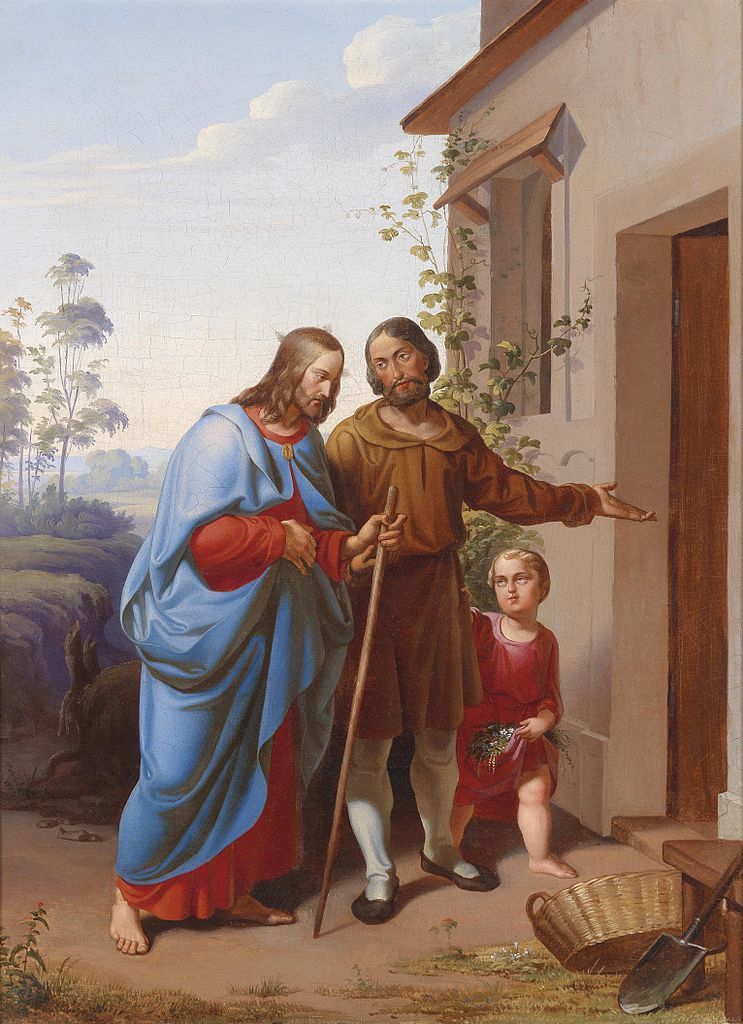
\includegraphics[width=0.95\textwidth]{images/illustrations/carlrahlchristushaus.jpg}
\end{center}